\documentclass[12pt,a4paper]{article}
\usepackage[utf8]{inputenc}
\usepackage{graphicx}
\usepackage{float}
\usepackage{subcaption}
\usepackage[margin=1in]{geometry}
\usepackage{hyperref}
\hypersetup{
  pdfborder = {0 0 0}
}
\usepackage[
backend=biber,
style=alphabetic,
]{biblatex}

\addbibresource{PhSp.bib}

\graphicspath{{./PhSp/}}
\DeclareGraphicsExtensions{.pdf,.jpeg,.jpg,.png}

\usepackage{amsmath} % equations
\usepackage{fancyhdr} % nicer page header

\setlength{\parindent}{0pt} % no paragraph indents
\setlength{\parskip}{1em} % paragraphs separated by one line

\newcommand\experiment{Photometry and Spectroscopy} %% experiment name
\newcommand\groupno{Group 3}       %%%%% group number
\newcommand\names{Pratyush Singh,\\
                  Proshmit Dasputpa\\}        %%%%% full names
\newcommand\expdate{19/03/2025}    %%%%% date of experiment day

\begin{document}
\begin{titlepage}
   \begin{center}
        \vspace*{3cm}
        \Huge{\experiment}
				
        \vspace{0.5cm}
        \LARGE{Lab course protocol}
				
        \vspace{3 cm}
        \Large{\groupno}
				
        \vspace{0.25cm}
        \large{\names}
				
        \vspace{2 cm}
        \Large{\expdate}
				
        \vspace{0.25 cm}
        \Large{Advanced lab course in astronomy\\
				Eberhard Karls Universit\"at T\"ubingen}
				
				\vspace{0.1 cm}
        \Large{WiSe 2024/25}
				
       \vfill
    \end{center}
\end{titlepage}

\pagestyle{fancy}
\fancyhf{}
\setlength{\headheight}{14.5pt}
\lhead{\groupno; \experiment}

%\section*{Abstract}
% This is optional, but never longer than half a page.

\tableofcontents
\newpage

\setcounter{page}{1}
\pagestyle{fancy}
\fancyhf{}
\rhead{\thepage}
\lhead{\groupno; \experiment}

\section{Introduction}\label{sec:intro} % labels allow references, particularly important for figures and tables
  In the experiment, we will use the 80 cm telescope of the IAAT to study photometry and spectroscopy. These two topics are fundamental to observational astronomy 
  and are used to study the properties of stars, galaxies and other bodies. In photometry, we aim to determine the brightness of several stars in the star cluster M37 in 
  the B and V filters which will be used to determine the age and distance to the cluster. In spectroscopy, we will look at the spectrum of one (or two) of the stars of 
  the Castor system and identify the $H\alpha$ spectral line (and more).

  In section \ref{sec:theory} we give a theoretical introduction to relevant topics like the working of CCD, photometry and spectroscopy. In section \ref{sec:80tele} we describe the 80 cm telescope
  used to obtain the data. In section \ref{sec:experiment} we describe the process of obtaining the data and then analysing the data seperately for photometry and spectroscopy.
\section{Theory}\label{sec:theory}
\subsection{Telescope}
  Telescopes are used in observing the EM radiation emitted by distant sources. They collect light from a certain direction and are used to apply an angular magnification to the image. The two major types of telescopes are 
  the lens telescope (the refractor) or the mirror telescope (the reflector). The amount of light that a telescope can gather depends on the `aperture' of the telescope $D$. The ratio of this and the focal length
  $F$ is the aperture ratio $F/D$. A telescope with a higher aperture ratio will produce a brighter image. The magnification of the telescope is determined by the ratio of the main mirror focal length $F$ and the eye piece focal length
  $f$. i.e. $M = F/f$. 
  \\
  The resolving power of a telescope is its ability to distinguish between two nearby sources and is defined by the Rayleigh criterion:
  \begin{equation}
    \alpha = 1.22 \frac{\lambda}{D}
  \end{equation}

  Unfortunately due to atmospheric effects, the resolving power is slightly worse and is limited to $\alpha = \lambda/D$. For a telescope with an aperture of 80 cm, the resolving power
  at $\lambda = 5700 \AA$  is \dots.
  \subsubsection{The 80 cm Telescope}
  \label{sec:80tele}
    The 80 cm telescope is located in Sand, Tübingen and was built in 2003. It is a mirror telescope in Cassegrain configuration with Nasmyth focus. It has an aperture of 80 cm and 
    a focal length of 6.4 m. For slewing, the telescope is mounted on an equatorial open fork mount and can move to focus on any point in the sky in its line of sight.
    \begin{figure}[H]
      \centering
      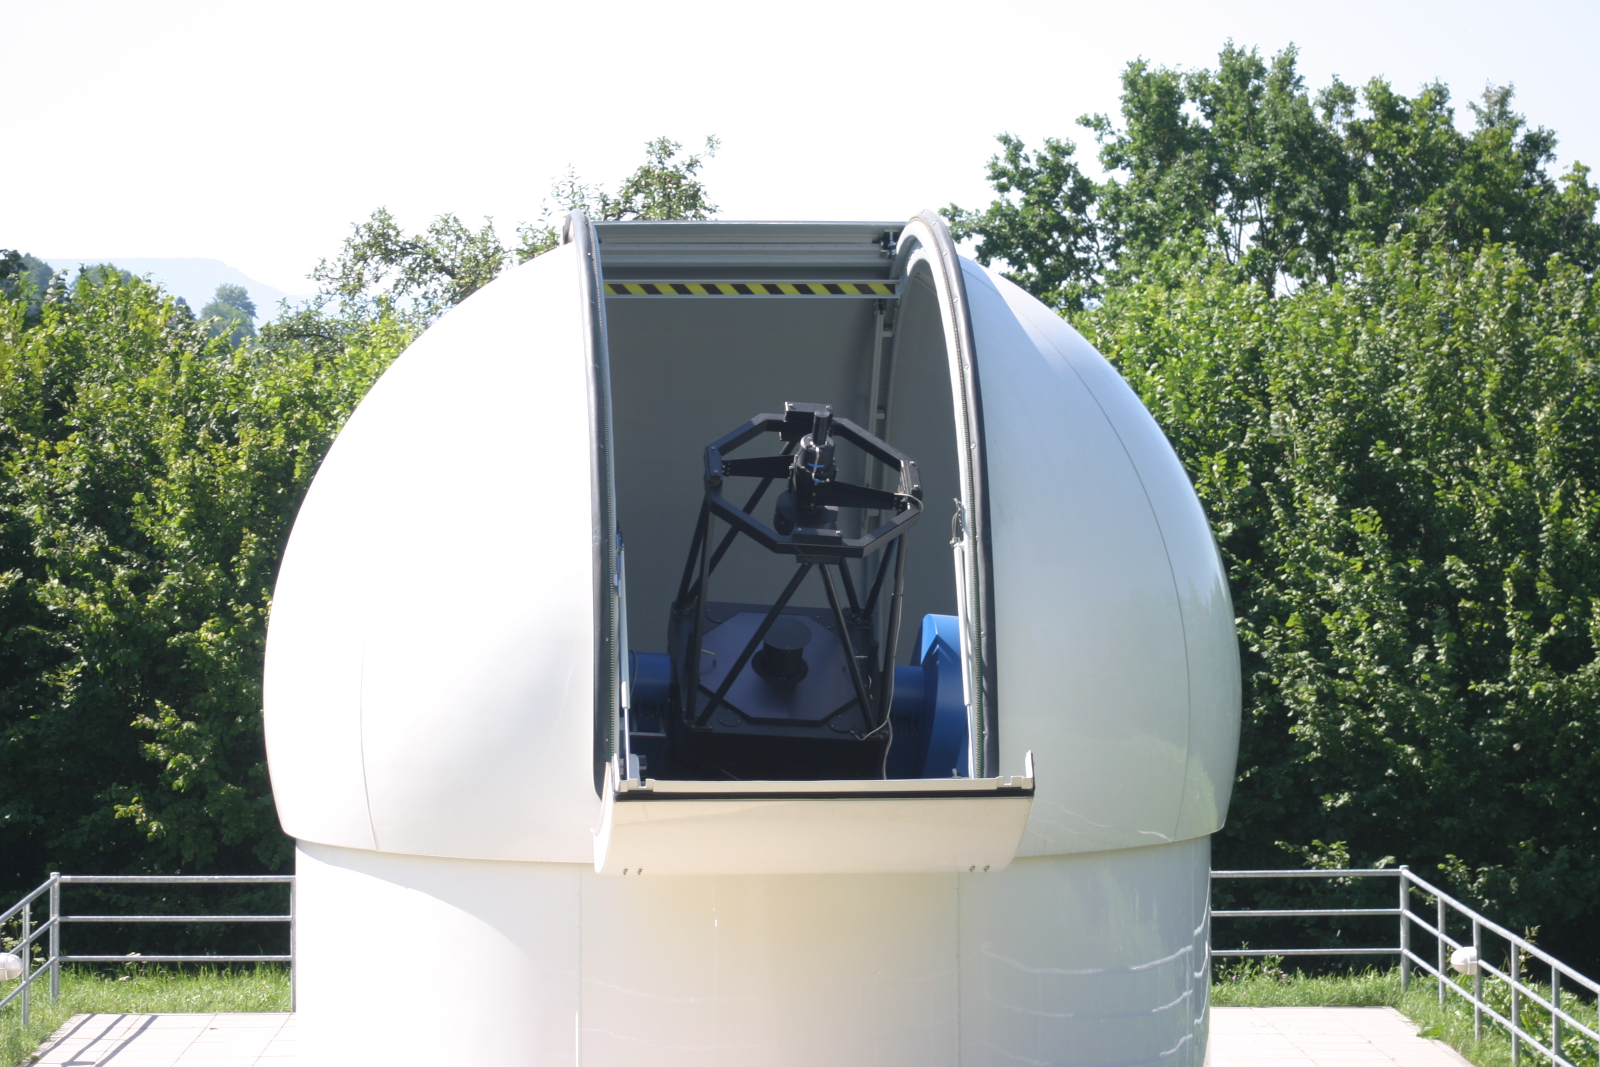
\includegraphics[width=0.5\textwidth]{./Pictures/2004_img_0962.jpg}
      \caption{The 80 cm telescope at the IAAT.}
      \label{fig:80cm}
    \end{figure}
    In figure \ref{fig:80cm_lp} we can see the path light has to travel to reach the focus points. The starlight enters from above and is reflected by the primary mirror towards the 
    secondary mirror. It reflects back the light towards a plain mirror which focuses the light on either the left or the right focus. This configuration (Cassegrain-Nasmyth) allows a smaller size of the telescope
    (around 3 m) for a larger focal length of 6.4 m. The Nasmyth focus also is beneficial for mounting heavy instruments that don't need to be moved with the declination axis. 
    \begin{figure}[H]
      \centering
      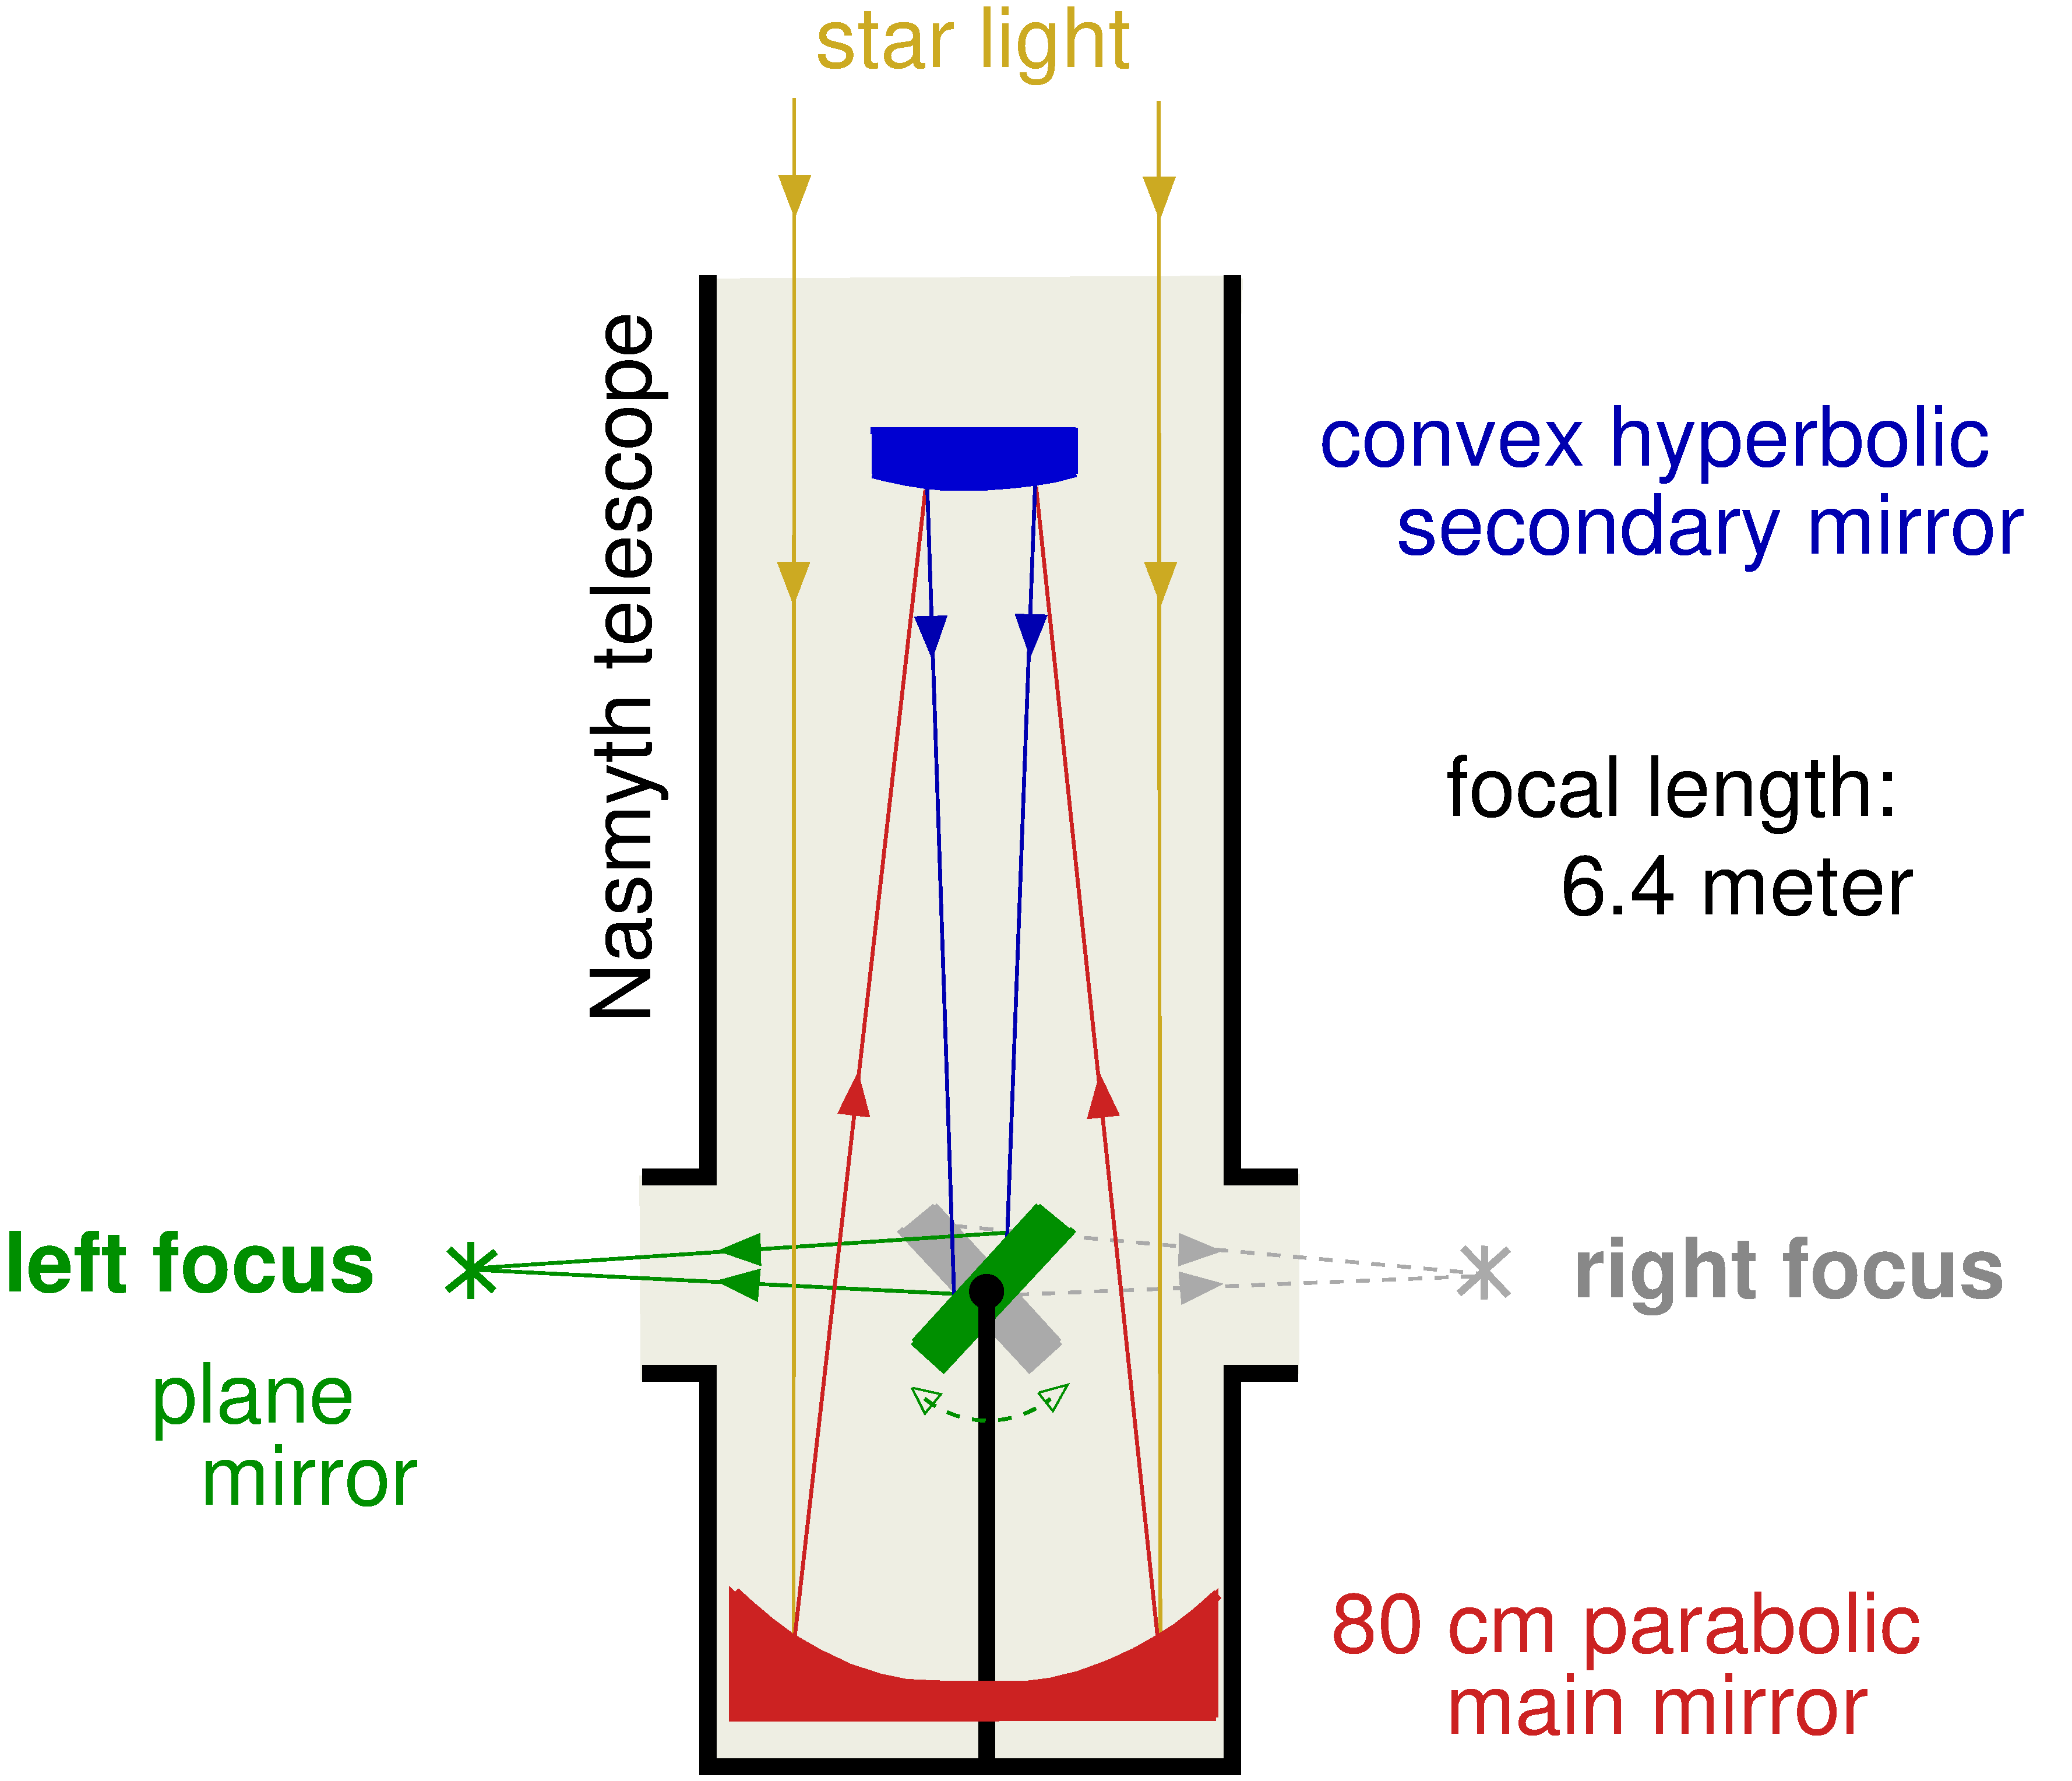
\includegraphics[width=0.5\textwidth]{Pictures/Nasmyth2.pdf}
      \caption{The light path of the 80 cm telescope.}
      \label{fig:80cm_lp}
    \end{figure}

  \subsection{CCD} 
  The Charge-Coupled Device (CCD) camera is a core component in astronomical imaging due to its high sensitivity and spatial resolution. In this experiment, the CCD camera is used to record both photometric and spectroscopic data with the 80 cm telescope at the IAAT.
  A CCD sensor consists of a two-dimensional array of photodiodes (pixels) embedded in a silicon semiconductor. When photons enter the silicon, they interact via the photoelectric effect, generating electron-hole pairs. The freed electrons are trapped in potential wells beneath electrodes, where they accumulate proportionally to the incident light intensity.
  The camera reads out the stored charges by shifting them line by line toward a readout register using precisely timed voltage sequences. These charges are then converted into voltages, amplified, and digitized by an analog-to-digital converter (ADC). This process (as shown in figure \ref{fig:CCD_block}) preserves the spatial distribution of the recorded light, forming a digital image.
  To suppress thermally induced noise (dark current), the CCD is cooled using a Peltier element. Additionally, dark-frame subtraction is applied to correct for background signals. For photometric observations, a motorized filter wheel is used to capture images in different wavelength bands (e.g., B, V, R), enabling color analysis and classification.
  Two cameras are used in the experiment:
  \begin{itemize}
    \item \textbf{SBIG STL-1001E}: A monochrome CCD with 1024×1024 pixels, a filter wheel, and Peltier cooling, optimized for photometry.
    \item \textbf{ZWO ASI294}: A color CMOS camera with 4144×2822 pixels and video capability, used for general imaging.
  \end{itemize}
  \begin{figure}[H]
    \centering
    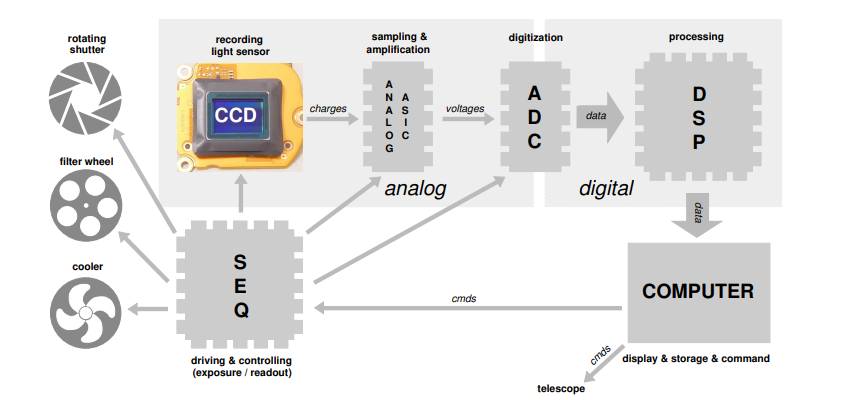
\includegraphics[width=1.0\textwidth]{Pictures/CCD.png}
    \caption{Block diagram of a typical CCD camera system.}
    \label{fig:CCD_block}
  \end{figure}
  The CCD camera's high full-well capacity and dynamic range make it especially suitable for capturing faint astronomical sources with precision, crucial for determining stellar brightness and spectral features.
 
 
  \subsection{Photometry}
  Photometry is the astronomical technique of measuring the brightness of celestial objects, such as stars and star clusters. Modern photometry uses electronic detectors and filters to quantify the light intensity in different wavelength bands.
  The observed brightness, or \textit{apparent magnitude}, is influenced by a star's distance, size, temperature, and luminosity. By comparing measurements across various color filters, photometry allows determination of a star's \textit{color index}, which is linked to its temperature and spectral class. Combined with theoretical models like the Hertzsprung-Russell Diagram (HRD) (Fig. \ref{fig:HR_Dia}), photometry helps estimate distances and ages of stellar populations.
  \begin{figure}[H]
    \centering
    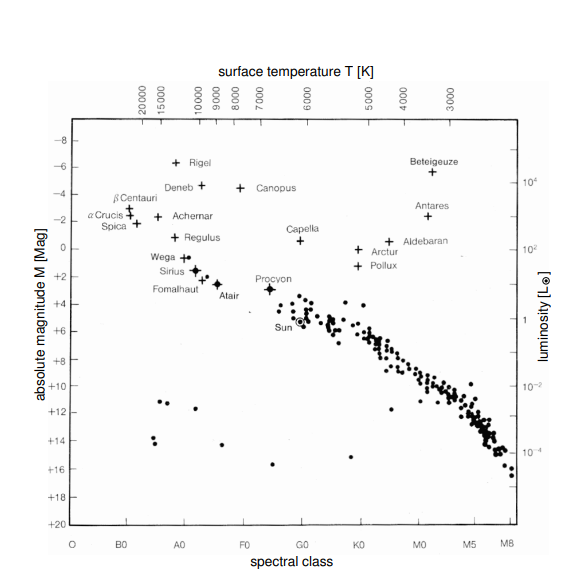
\includegraphics[width=1.1\textwidth]{Pictures/HRD.png}
    \caption{Hertzsprung-Russel diagram of night sky stars (Credit: Karttunen and Kröger et al., 1987).}
    \label{fig:HR_Dia}
  \end{figure}
  \subsubsection*{Photometric Techniques in the Experiment}
  In this experiment, photometric data is collected using the \textbf{SBIG STL-1001E CCD camera}, a high-sensitivity monochrome sensor equipped with a motorized filter wheel. The camera is mounted at the Nasmyth focus of the 80 cm telescope at the IAAT.
  The following steps summarize the photometric technique used:
  \begin{itemize}
    \item \textbf{Multi-band Imaging:} The CCD captures images of a star cluster through standard Johnson filters (typically $B$, $V$, and $R$), allowing for determination of magnitudes in different wavelength bands.
    \begin{table}[h!]
      \centering
      \caption{The color filters of the Johnson system}
      \begin{tabular}{|c|l|c|}
      \hline
      \textbf{Symbol} & \textbf{Color} & \textbf{Wavelength $\lambda_\mathrm{eff}$ [\AA]} \\
      \hline
      U & Ultra violet & 3500 \\
      B & Blue         & 4350 \\
      V & Visual       & 5550 \\
      R & Red          & 7100 \\
      I & Infrared     & 9700 \\
      \hline
      \end{tabular}
      \end{table}
      
    \item \textbf{Dark Frame Subtraction:} To remove thermal noise, a dark image is taken with the shutter closed and subtracted from the light-exposed images.
    \item \textbf{Flat-Field Correction:} To correct for pixel-to-pixel sensitivity variations, a uniformly illuminated image (flat field) is used to normalize the response.
    \item \textbf{Aperture Photometry:} The brightness of stars is determined by summing the pixel values within a defined aperture around each star and subtracting the background.
    \item \textbf{Color-Magnitude Diagram (CMD):} Using the measured magnitudes, a CMD is plotted to analyze the properties of the star cluster. The CMD allows determination of the cluster’s distance and age by fitting theoretical isochrones.
  \end{itemize}
  This method enables precise brightness measurements and color analysis, which are essential for stellar classification and cluster analysis.





  \subsection{Spectroscopy}
    Studying the spectrum of stars can reveal information like their temperature, composition and their physical properties. The absorption and emission lines present 
    in a spectra caused by certain transitions in the elements present in the star and help in identifying its chemical composition. These lines are used to group
    stars into different spectral classes. \\

    \subsubsection{Star Classification}
    Using the Morgan and Keenan system, stars are classified depending on their spectrum and their luminosity. Both these parameters are required for classification since 
    stars st different stages of their life can have the same spectral class, while their sizes may strongly differ. Therefore to make their classification unambiguous `luminosity class' 
    is also used. The luminosity classes are defined in the figure \ref{fig:MK}.
    \begin{figure}[H]
      \centering
      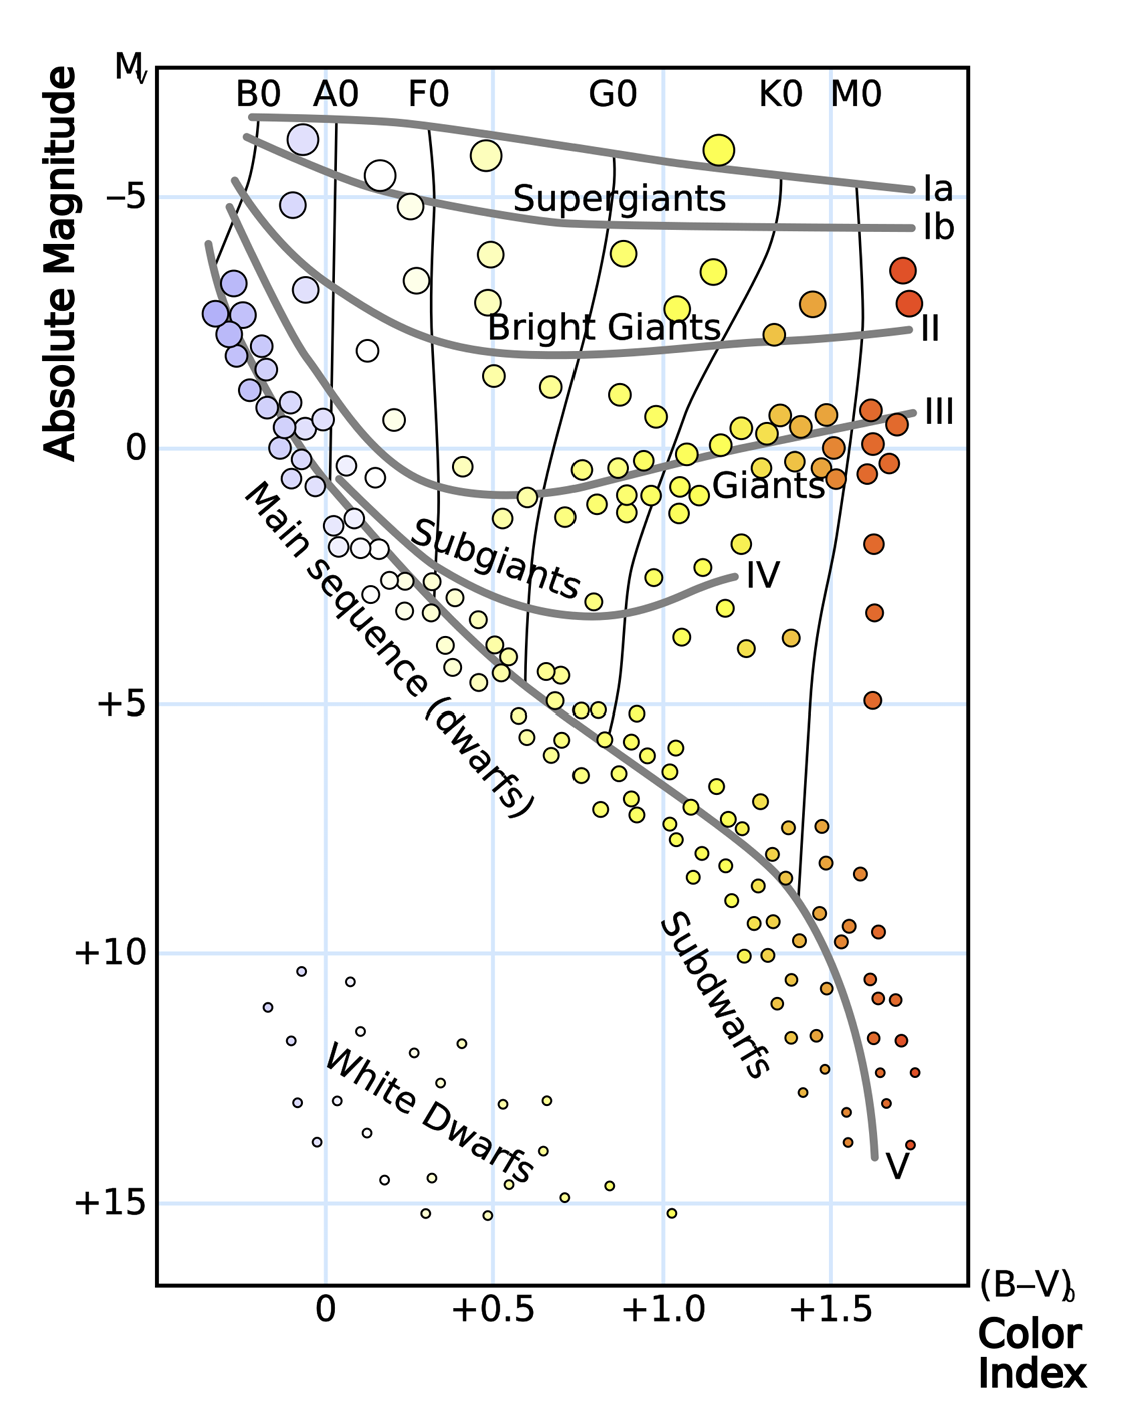
\includegraphics[width=0.5\textwidth]{Pictures/HRD_lum_class.png}
      \caption{HRD diagram with Luminosity Classification}
      \label{fig:MK}
    \end{figure}

    Stars are classified into a `spectral class' based on the strength of their various spectral lines. The spectral class of a star is also a direct measure of the temperature of the star. The spectral classes are labelled
    `O', `B', `A', `F', `G', `K', `M', `L' and `T' in decreasing order of temperature. Each is further split into 10 sub classes from 0 to 9. \\
    \begin{table}[H]
      \begin{tabular}{||c|c|c||}
        \hline
        Spectral Type & Temperature Range (K) & Distinguishing Features\\
        \hline
        \hline
        O	& \textgreater 25,000K	&H; HeI; HeII\\
        B	&10,000-25,000K	&H; HeI; HeII absent\\
        A	&7,500-10,000K	&H; CaII; HeI and HeII absent\\
        F	&6,000-7,500K	  &H; metals (CaII, Fe, etc)\\
        G	&5,000-6,000K  	&H; metals; some molecular species\\
        K	&3,500-5,000K	  &metals; some molecular species\\
        M	&$\leq $3,500K	metals;& molecular species (TiO!)\\
        C	&$\leq $ 3,500K	metals; &molecular species (C2!)\\
        \hline
      \end{tabular}
      \caption{Temperature and Absorption lines at different spectral Classes\cite{Spectral_Classification}}
    \end{table} 
    Stellar plasma below the photosphere creates a black body spectrum. The temperature at which this peaks is the effective temperature of the star. As the temperature in the outer regions of the photosphere is lower,
    different elements absorb parts of the light coming from deeper in the star and create the absorption lines. These lines are highly dependent on the effective temperature and the elements present in the photosphere.
    \\
    The most abundant absorption lines are usually the $H_\alpha$, $H_\beta$, $H_\gamma$ and $H_\delta$ lines of the Balmer series. These are caused by ionized hydrogen, which is the most abundant elements in stars.
    Hydrogen lines are most abundant in A type stars. For G type and cooler stars, Calcium lines are more dominant. Figure \ref{fig:abs_lines} shows this in more detail.
    \begin{figure}[H]
      \centering
      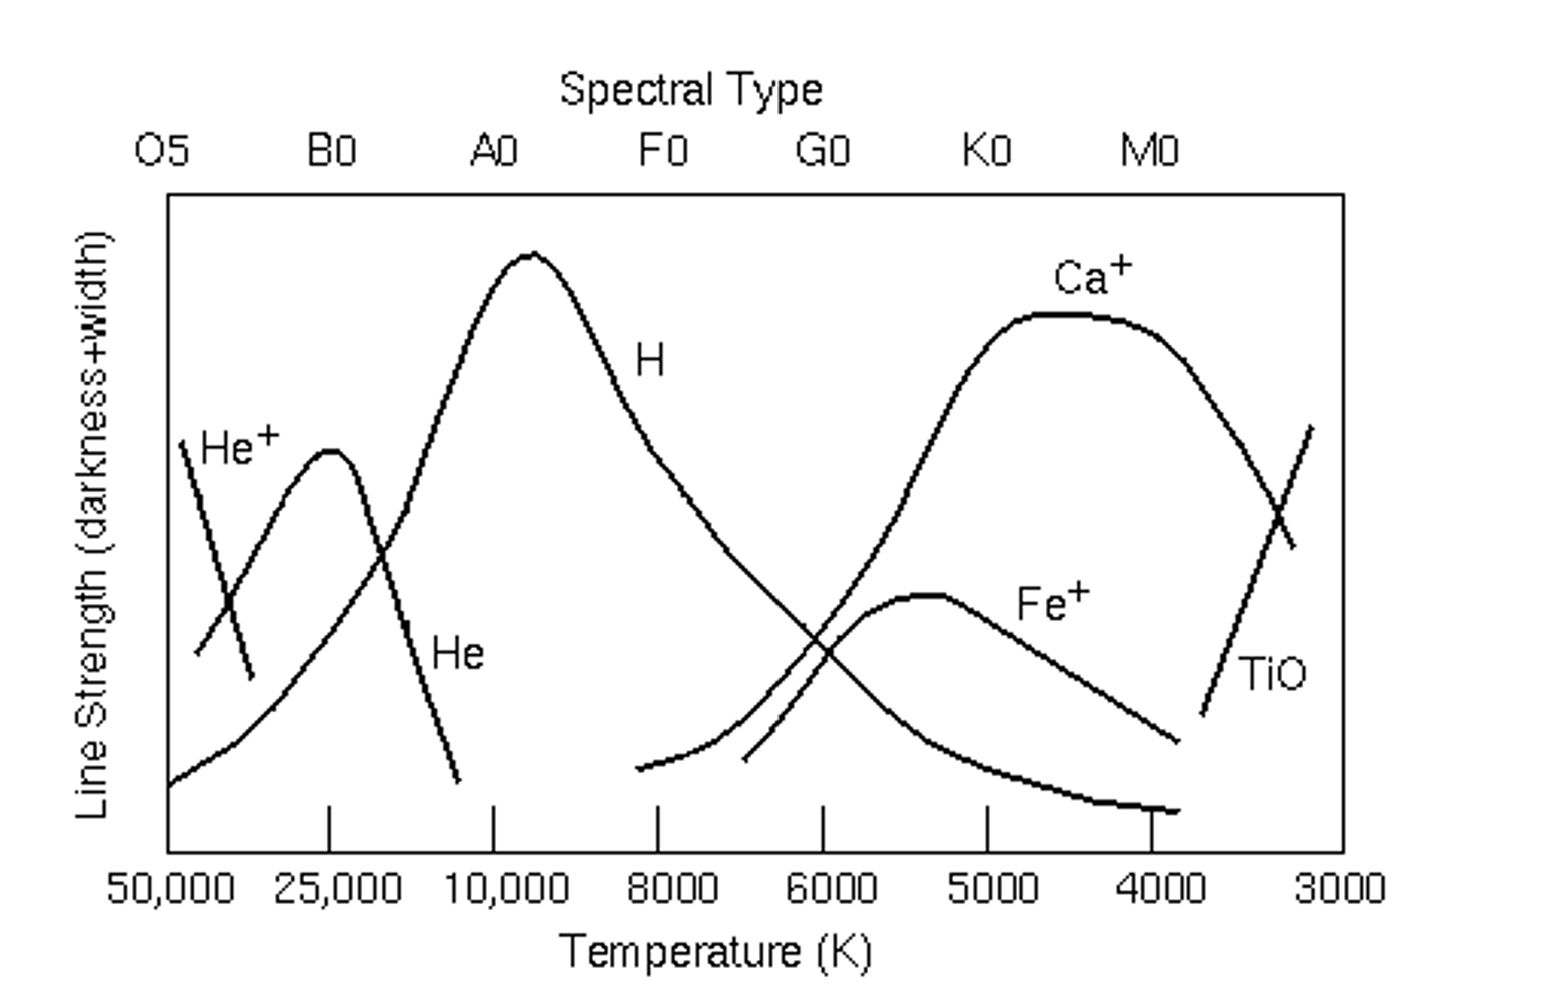
\includegraphics[width=0.75\textwidth]{Pictures/Line_strength.png}
      \caption{Strength of absorption lines at different temperatures}
      \label{fig:abs_lines}
    \end{figure}
    Figure \ref{fig:spec_class} shows the spectra of stars of different sizes. Most of the spectral features are found in UV, hence spectroscopy is very popular in UV astronomy. 
    
    \begin{figure}[H]
      \centering
      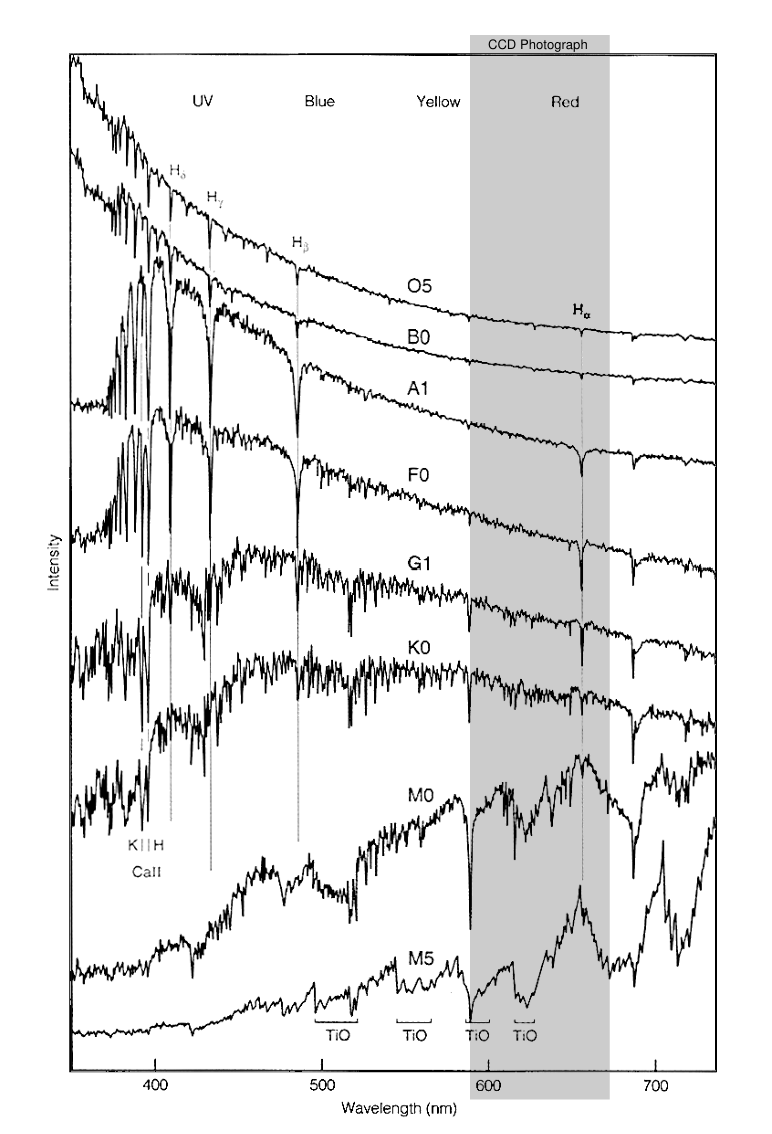
\includegraphics[width=0.75\textwidth]{Pictures/Spectral_class.png}
      \caption{Spectra of stars of different spectral classes.}
      \label{fig:spec_class}
    \end{figure}
\section{Experiment} 
\label{sec:experiment}
\subsection{Photometry}
For the photometric experiment, the CCD camera SBIG STL1001 was mounted to
the left focus of the 80 cm telescope. The camera had a filter wheel, which was controlled by the Maxim-DL software on the Navigation and Observation Computer.
For the photometric analysis, a \texttt{BLUE} and a \texttt{GREEN} image of the open star cluster \textbf{M37} was photographed.
\subsubsection{Recording steps}
The following steps were performed during the recording phase of the photometric experiment:

\begin{enumerate}
    \item \textbf{Telescope Setup:} The 80 cm telescope was aligned and slewed to the target star cluster using the equatorial mount and control software.
    
    \item \textbf{Camera Initialization:} The SBIG STL-1001E CCD camera with integrated filter wheel was mounted at the Nasmyth focus. The Peltier cooling system was activated to reduce thermal noise.
    
    \item \textbf{Focusing:} A bright reference star was used (in our case, \textbf{Capella}) to focus the telescope. Short test exposures were taken to check the sharpness of the star image.
    
    \item \textbf{Image Framing:} The target (\textbf{Star cluster :} \texttt{M37}) was centered in the CCD field of view using short exposures (usually 10 seconds) and manual fine adjustments of the telescope tracking (For example, changing the telescope focus until the best focal number was found).
    
    \item \textbf{Filter Selection:} Color filters from the Johnson system ($B$(Blue), $G$(Green)) were selected. The filter wheel was rotated to place the appropriate filter in front of the CCD. The two images were successfully photographed.
    
    \item \textbf{Data Storage:} Both images were saved in \texttt{FITS} format and labeled with relevant metadata (filter, exposure time, object name) for later analysis.
\end{enumerate}
\subsubsection{Analysis of the data}

The following steps were performed during the analysis phase of the photometric experiment:

\begin{enumerate}
    \item \textbf{Starting the ZAMS Analyser:} The IDL/GDL-based software is launched to begin the guided photometric analysis process.

    \item \textbf{Selecting the Calibration Stars:}  5 calibration stars are identified and clicked on in both the BLUE and GREEN FITS images. These stars are used for filter correction.

    \item \textbf{Retrieval of Standard Magnitudes:} The $B$ and $V$ magnitudes for the selected stars are obtained from the WEBDA online database.

    \item \textbf{Recording of Measured Magnitudes:} Using the ZAMS-Analyzer, the $B$ and $V$ magnitudes of the same 5 stars are measured and recorded from the FITS images.

    \item \textbf{Correction Calculation:} The average differences between the recorded and literature magnitudes is computed to determine $\Delta B$ and $\Delta V$ correction values.

    \item \textbf{Application of Color Corrections:} $\Delta B$ and $\Delta V$ is entered into the ZAMS-Analyzer to calibrate the BLUE and GREEN images to the standard Johnson filter system.

    \item \textbf{Aligning the Images:} The coordinates of the BLUE and GREEN images are matched by selecting the same star in both images. The software adjusts for any offset.

    \item \textbf{Selecting the Cluster Stars:} Stars belonging to the cluster in both corrected images are identified and clicked on. At least 30–40 stars should be selected for a meaningful CMD. We have selected roughly about 130 stars for our analysis.

    \item \textbf{Generation of the CMD:} The software plots a Color-Magnitude Diagram (CMD) using the corrected $B - V$ color index and $V$ magnitude.

    \item \textbf{Determination of Cluster Distance:} The observed CMD is vertically fitted to the theoretical Zero-Age Main Sequence (ZAMS) and the distance modulus $(V - M_V)$ is used to calculate the distance to the cluster.

    \item \textbf{Determining the Cluster Age:}
    \begin{itemize}
        \item \textbf{Turn-Off Method:} Identification of the brightest star that has turned off the main sequence and estimating the cluster age from its position.
        \item \textbf{Isochrone Method:} Fitting the CMD to a theoretical isochrone curve and reading off the age from the best-fitting model.
    \end{itemize}
\end{enumerate}

\subsubsection{Results}
\begin{figure}[H]
  \centering
  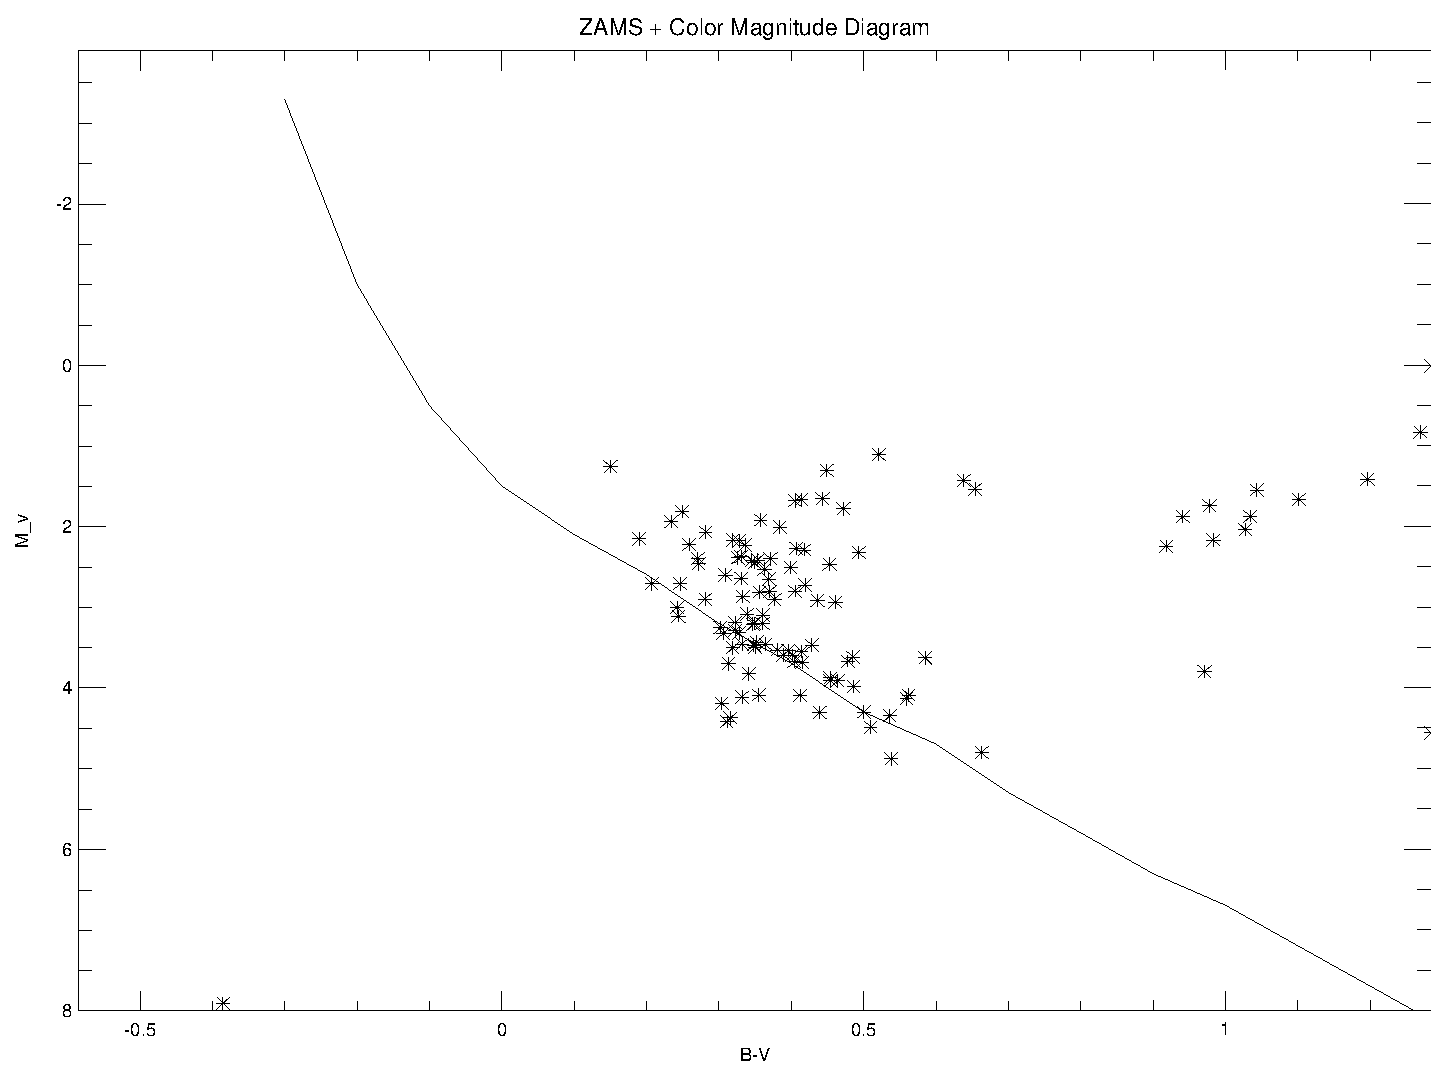
\includegraphics[width=1.0\textwidth]{Pictures/CMD_M37_2.pdf}
  \caption{Color-Magnitude Diagram Calibrated with ZAMS Diagram}
  \label{fig:CMD_ZAMS}
\end{figure}

\subsubsection*{Determination of distance to cluster}
The \textbf{distance modulus} is adjusted iteratively - such that the stars in the lower end of the CMD touch the ZAMS. 
\\ Adhering to the software's instructions, we have chosen $(V - M_V)$ to be \texttt{12}. The resulting plot is shown in figure \ref{fig:CMD_ZAMS}.
\\ The distance of the open cluster M37 is estimated to be around 2511 Parsec. If we take into account the \textbf{extinction factor} then the distance comes out to be roughly \fbox{1655 Parsec}.
\\ This value is close to \textbf{ 1383 Parsec}, which is the official WEBDA data for our target star cluster M37. The difference is around 300 Parsec, which is to be expected as the data we are working with might contain some errors. 
\\ One of such errors involve the selection of stars which might be far away from the target cluster - even if they seem to be a part of the cluster.
\subsubsection*{Determination of age of cluster}
\begin{figure}[H]
  \centering
  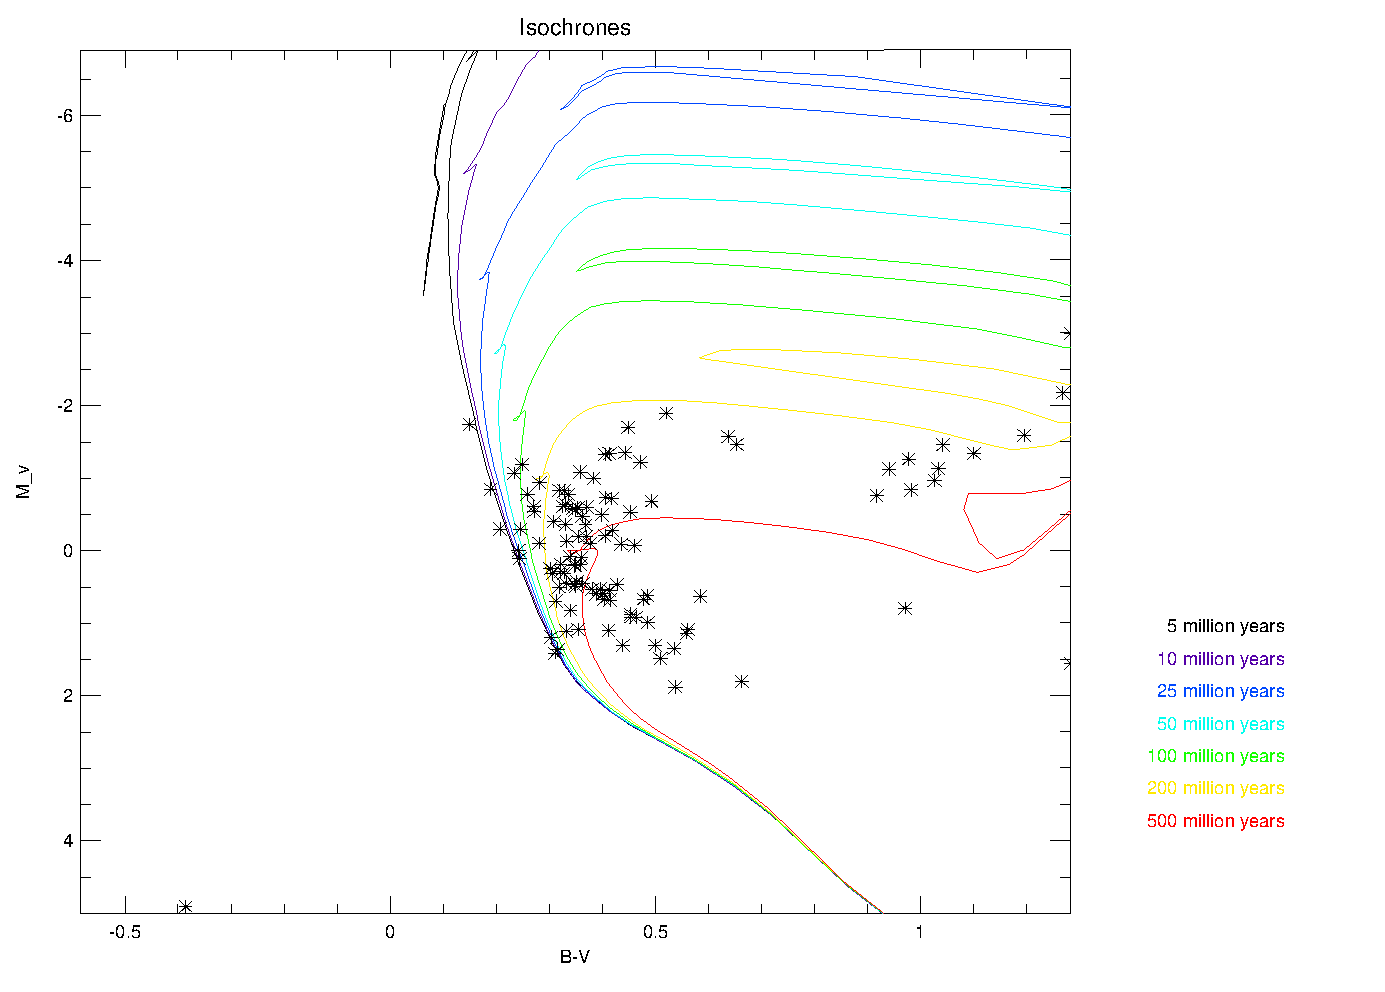
\includegraphics[width=1.0\textwidth]{Pictures/ISO_M37_2.pdf}
  \caption{ Color-Magnitude Diagram Calibrated with Isochrone Diagram}
  \label{fig:CMD_ISO}
\end{figure}

To estimate the age of the cluster we can use the \textbf{isochrone fitting method}. Isochrones are lines of constant age calculated from stellar evolution models. We just fit our CMD to the Isochrone Diagram (Fig. \ref{fig:CMD_ISO}) to estimate the age.
\\ The age of the cluster is estimated to be around \fbox{720 million years}. In the WEBDA data, the age of the cluster is given to be around \textbf{ 350 million years} - which is a significant difference from our result.
\\ One reason for this discrepancy could be an insufficiently large sample size of stars while plotting the Color-Magnitude Diagram. Another possibility is the same error faced while determining the distance to the M37 cluster, that is unintentionally choosing stars which do not belong to our target cluster.


\subsection{Spectroscopy}

    We observed the spectrum of one (or both) stars in the Castor binary system. To observe the spectra, the 10C spectrograph was mounted on the 
    left focus of the 80 cm telescope. The spectrograph uses a CCD camera to obtain the spectral image of the star. To control the spectrograph, `Maxim DL'
    software is used. 
    \subsubsection{Recording the Data}
      In order to obtain the spectra, the steps are listed below:
      \begin{enumerate}
        \item The telescope is powered on and the operation software is started on the `Telescope Computer', `Navigation and Observation Computer' and the `Spectral Analysis Computer'.
        \item The calibration lamps and the CCD of the spectrograph are powered on.
        \item Adjust the focus of the CCD. This must be set up manually directly at the spectrograph by following the markings on the camera. When mounting the spectrograph, be careful not To
              touch the focus dial.
        \item The telescope is slewed to the target star. Out of focus, the star will appear as a donut shaped object. The focus is manually adjusted until we observe a star like object(s).
        \item When the calibration lamps are on, the slit is visible between the two red discs that appear in the eyepiece. The telescope is slewed slightly until one of the stars is directly on the slit. 
        \item The spectral image can now be taken by the spectrograph. 
      \end{enumerate}

      \begin{figure}[H]
        \centering
        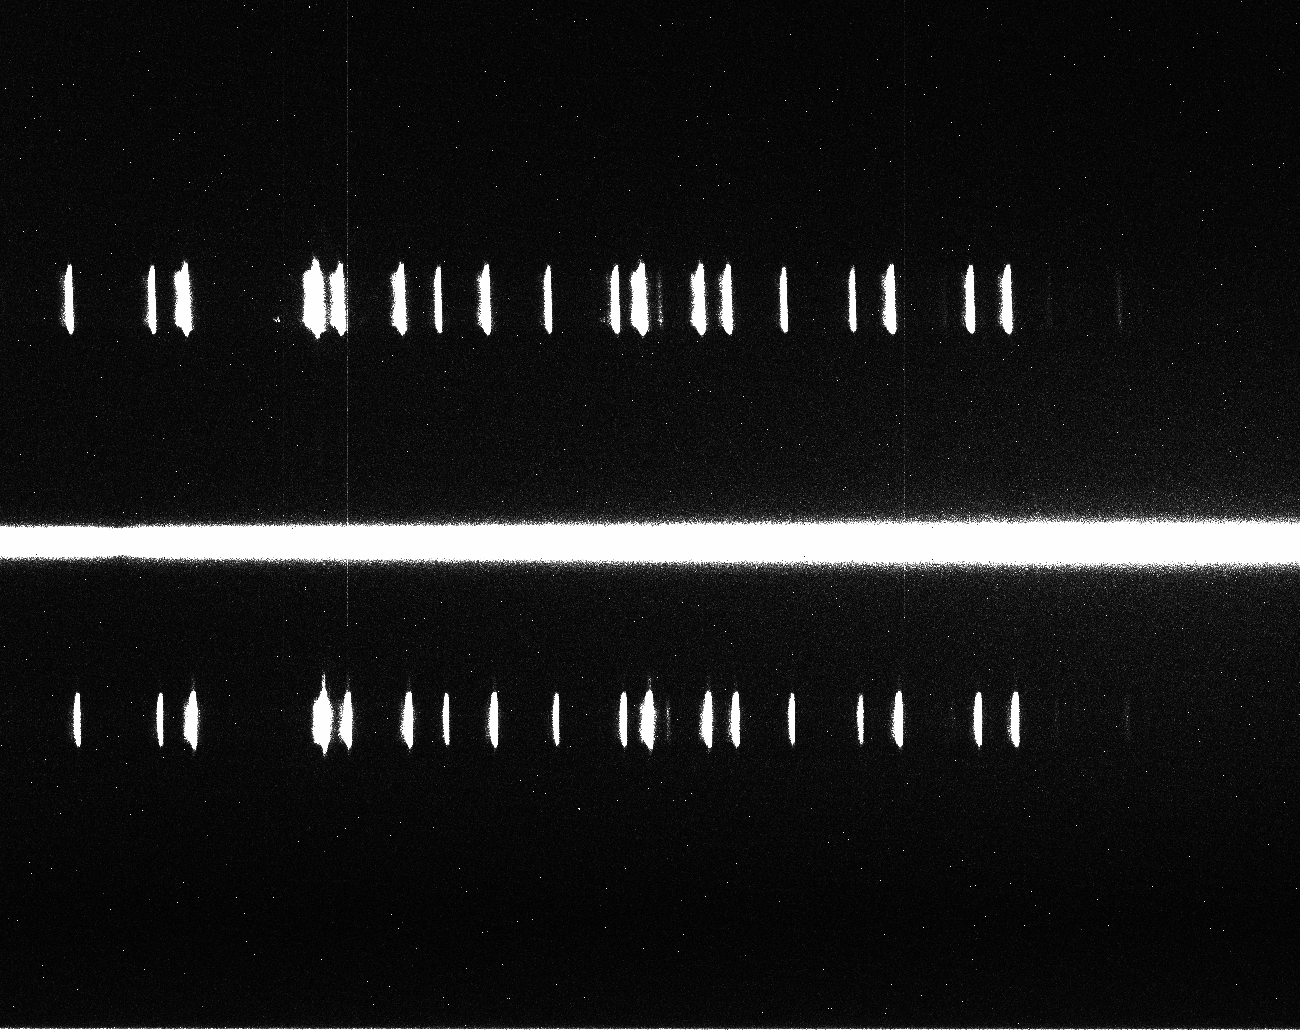
\includegraphics[width=0.75\textwidth]{Pictures/spectrum_image.png}
        \caption{Spectral image of the Castor binary system obtained using the SX-HX9 CCD camera of the 10C spectrograph and the 80 cm telescope. 
        We observe the top and bottom calibration lines and the star spectrum in the middle. Not much is directly visible in the image except possibly the $H_\alpha$ line}
        \label{spectrum_img} 
      \end{figure}
    \subsubsection{Data Analysis}
      The obtained spectral image is analysed using the `Spec-Analyzer' software. The software interactively guides the user through the steps to analyze the image. The software is written In
      IDL/GDL and involves command line inputs and mouse pointer interactions. Care needs to be taken when clicking mouse buttons as it can send incorrect inputs to the software. If a mistake is made, the process
      needs to be started again. \\
      In figure \ref{spectrum_img} The top and bottom spectrums are created by Neon lamps and are used for calibration of  the star spectrun. Currently, the star spectrum appears as a
      continuous bright band in the middle and only a small decrease in intensity near what is possibly the $H_\alpha$ line is visible. \\
      Using spec-analyzer, the final spectra is obtained with the following steps:
      \begin{enumerate}
        \item The software scans for three traces from the image, the top and bottom calibration traces(\texttt{cal-trace1} and \texttt{cal-trace2}) and the middle trace for the star (\texttt{spec-trace}). A `trace' is a 
              1-D array that contains all the pixel values along the x direction for a fixed y. For `spec-trace', we take average of several traces along the middle region which covers the star spectrum. 
        \item We now obtain the raw uncalibrated spectrum.
          \begin{figure}[H]
            \centering
            \begin{subfigure}{0.49\textwidth}
              \centering
              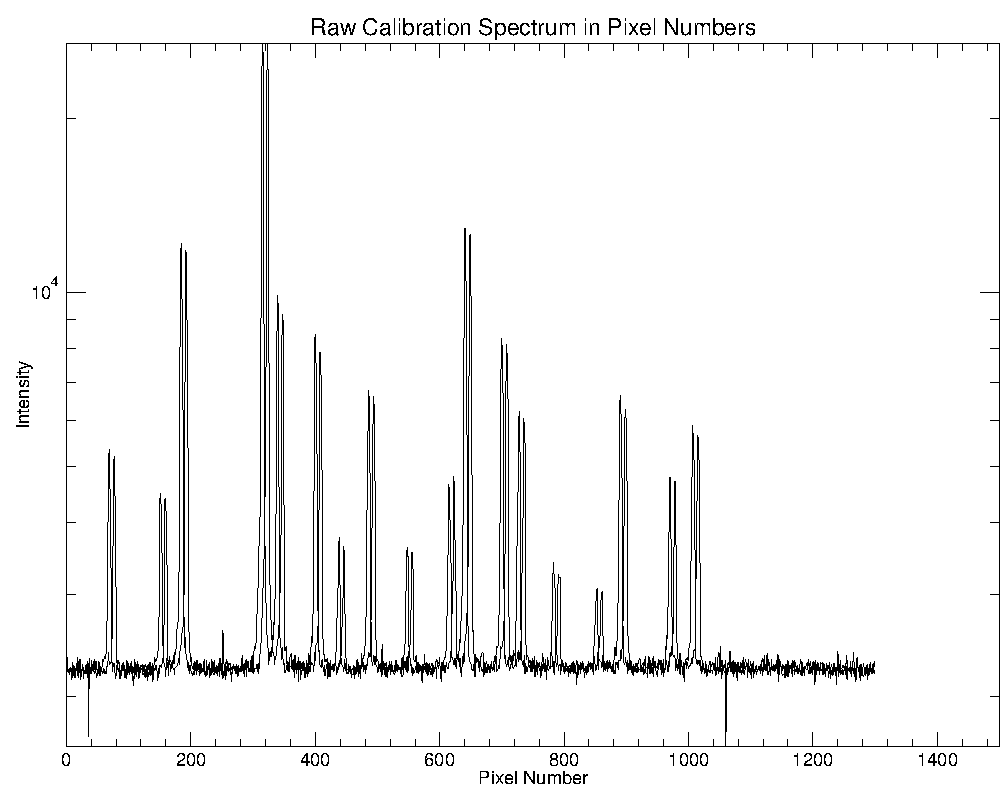
\includegraphics[width=3in]{Pictures/Castor_121sec_2025_2-CalRawSpec.pdf}
              \caption{Raw calibration spectrum}
              \label{fig:rawcalspec}  
            \end{subfigure}
            \begin{subfigure}{0.49\textwidth}
              \centering
              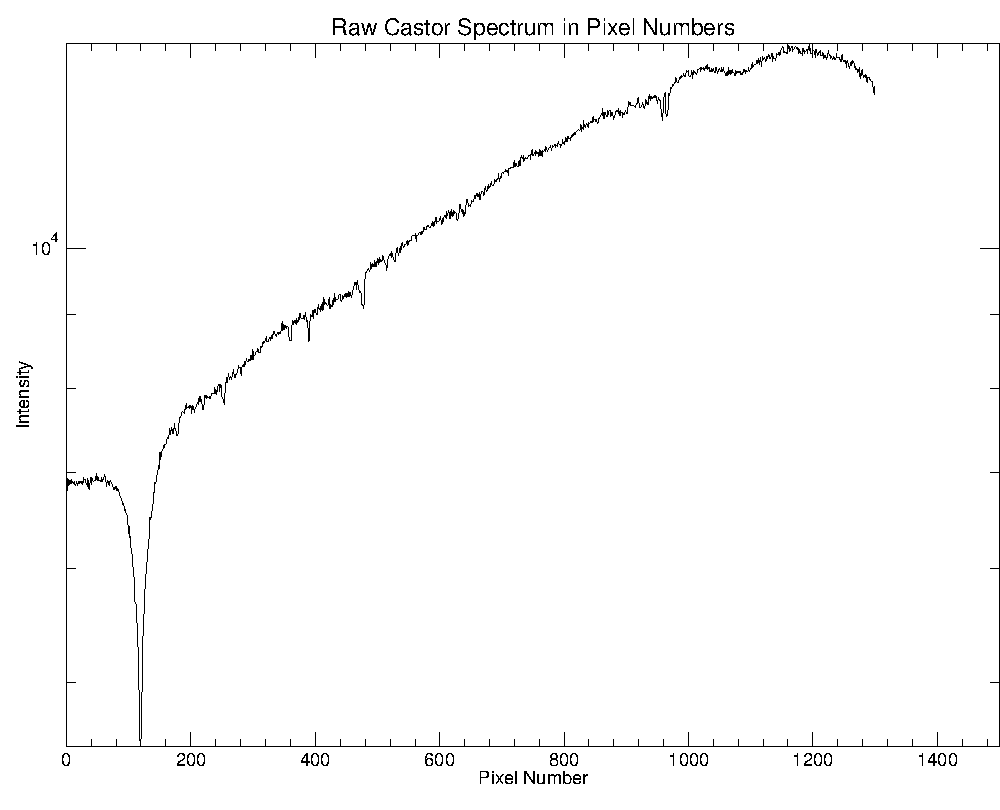
\includegraphics[width=3in]{Pictures/Castor_121sec_2025_2-RawSpec.pdf}
              \caption{Raw star spectrum}
              \label{fig:rawstarspec}
            \end{subfigure}
            \caption{The raw spectrum with the pixel number on the x axis and the intensity on the y axis. }
          \end{figure}

        \item Due to the CCD camera being removable, there will be a skew between the image plane and the x axis of the spectrograph which needs to be corrected for. This can be done by correlating both the calibration spectrums
              and the maximum correlation can be observed manually and is sent as an input to the software. Here, it was found to be $0.8$.
        \item Now, we need to calibrate the observed calibration spectra to a reference spectrum with the same Neon lines. This is difficult to do hence we will compare
              the observed spectrum image with a calibrated spectrum image. This calibrated image is shown in figure \ref{fig:calibrated_cal_image}.
              \begin{figure}[H]
                \centering
                
\includegraphics[width=0.95\textwidth]{Pictures/ReferenceImage.pdf}
                \caption{Calibrated spectrum image. This was recorded using earlier using the 10C spectrograph calibration lambs for lines in optical spectrum($4000\AA-8000\AA$ ) These lines are compared with the observed calibration spectrum in figure \ref{spectrum_img}}
                \label{fig:calibrated_cal_image}
              \end{figure} 
        \item We manually compare both these images to get the wavelengths of any 5 matching lines in the observed spectrum. This will finally convert the pixel numbers to wavelength numbers. If chosen correctly, the graph of wavelength vs pixel numbers would be a straight line.
        \item We now have the calibrated spectrum
              \begin{figure}[H]
                \centering
                \begin{subfigure}{0.49\textwidth}
                  \centering
                  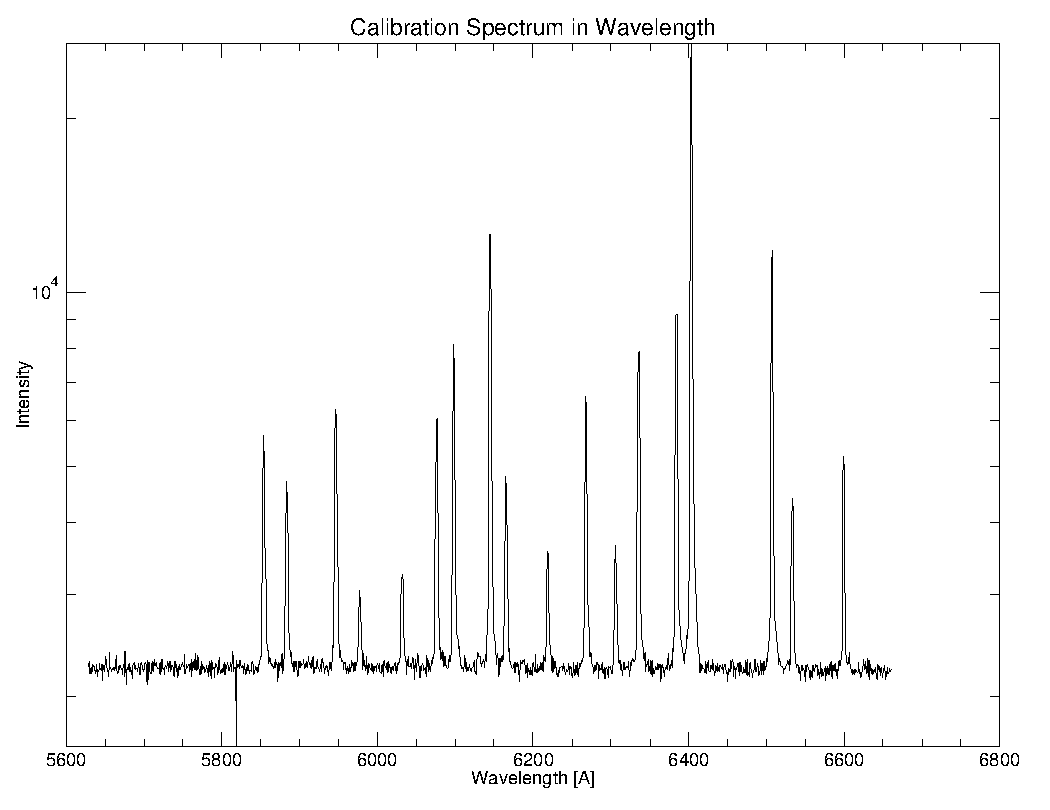
\includegraphics[width=3in]{Pictures/Castor_121sec_2025_2-CalSpectrum.pdf}
                  \caption{Calibrated spectrum for observed calibration lines}
                  \label{fig:calibrated_calspec}
                  
                \end{subfigure}
                \begin{subfigure}{0.49\textwidth}
                  \centering
                  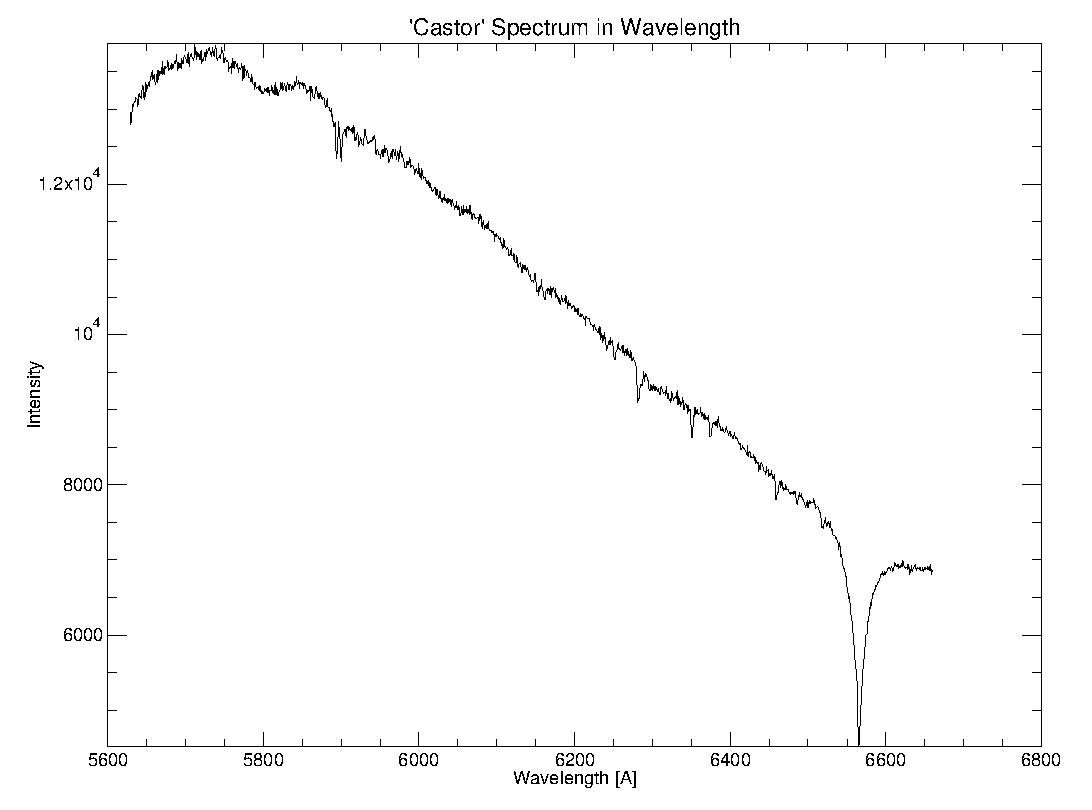
\includegraphics[width=3.4in]{Pictures/Castor_121sec_2025_2-Spectrum.pdf}
                  \caption{Calibrated star spectrum}
                  \label{fig:calibrated_starspec}
                \end{subfigure}
                \caption{The calibrated spectrum with the wavelength on the x axis and the intensity on the y axis}
              \end{figure}
      \end{enumerate}

    \subsubsection{Results}
      Comparing the observed spectra in figure \ref{fig:calibrated_starspec} from the spectrum of stars in various spectral classes in figure \ref{fig:spec_class} we see that it best matches that of a 
      type A star. This is indeed the case. Castor is a system of six stars in three spectroscopic binary systems. The two brightest stars observed by the 80 cm telescope (Castor Aa and Castor Ba) are type A stars (A1V and Am respectively).\cite{Wikipedia_contributors_2025}\cite{Pourbaix_Tokovinin_Batten_Fekel_Hartkopf_Levato_Morrell_Torres_Udry_2004}
      \begin{figure}[H]
        \centering
        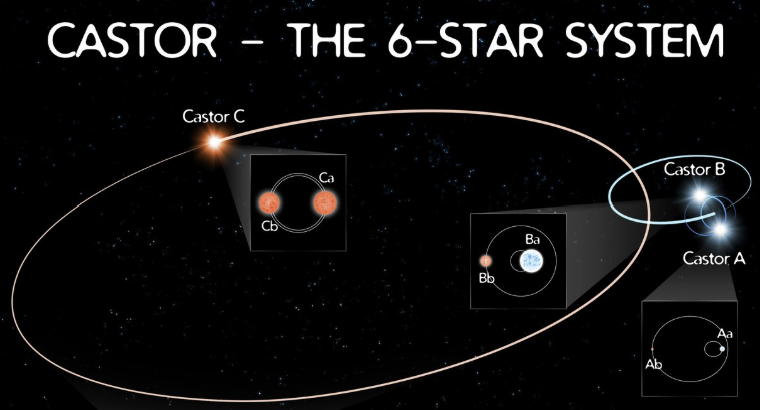
\includegraphics[width=0.75\textwidth]{Pictures/Castor.png}
        \caption{Diagram of the Castor system. Courtesy NASA/JPL-Caltech\cite{Wikipedia_contributors_2025}\cite{Castor}}
        \label{fig:comparison}
      \end{figure}

      Looking closely at the spectrum in figure \ref{fig:calibrated_starspec} and using a digital ruler, we roughly find the most prominent absorption lines at $\sim 5900 \AA$(two lines close by), $\sim 6280 \AA$, $\sim 6350 \AA$, $\sim 6375 \AA$, $\sim 6460 \AA$ and the most prominent line 
      being located at $\sim 6563 \AA$. This is the $H_\alpha$ line formed due to the Balmer transition in neutral H. This is present in large quantities in all main sequence stars.\\
      Two lines close by, likely at $5890 \AA$ and $5896$ AA could be the sodium doublet lines originating from neutral sodium. Comparing with lines on the NIST database, these had the highest relative intensity.\cite{NIST_ASD} This could be present in the star atmosphere. \\
      The line close to $6280 \AA$ could be caused by $O_2$ in the earth's atmosphere and is not a part of the star's spectra. \\

      Looking at the NIST database, the line with the largest relative intensity close to $6350 \AA$ is from neutral Vanadium. This could possibly be present in the star's atmostphere.\\ 

      The peak near $6375 \AA$ could be the $6363 \AA$ neutral oxygen line in stellar spectra.\\

      The peak near $6460 \AA$ could be the neutral iron line. It appears blended with another spectral line close by. 



\section{Conclusions}
We have estimated the distance of the M37 open cluster with some accuracy. However, the error in the age of the cluster is determined to be quite significant. The reasons might be a shorter sample size of stars (than what is required), or some kind of manual error in the calibration process.

\setcounter{secnumdepth}{0}

\printbibliography
\appendix
\section{Appendix}

Please attach here your original handwritten notes and other documents created during the experiment.

\end{document}

